\section{Introduction}
\begin{figure}[t]
\centering
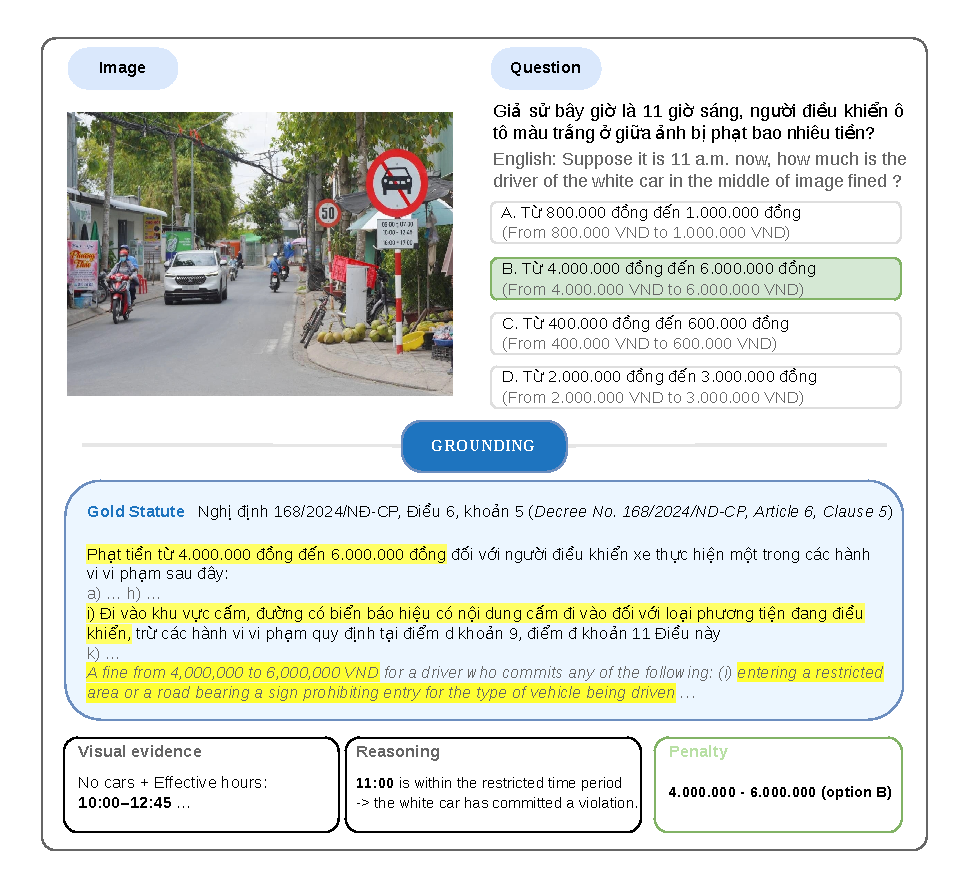
\includegraphics[width=\linewidth]{Figures/Sample2.pdf}
\caption{
An example from \textsc{ViTALBench}. The grounding shown is provided only for illustration and is not part of the benchmark annotations.
}
\label{fig:sample}
\end{figure}
Recent advances in vision-language models (VLMs)  have significantly enhanced their ability to perceive and reason about complex traffic environments~\cite{zhou2024vision}. Nevertheless, recognizing a traffic violation is fundamentally different from understanding a traffic scene. It requires reasoning beyond visual recognition. A model must understand the traffic context, identify potential violations, link its judgment to relevant legal provisions, and determine the associated legal consequences. Despite impressive progress in intelligent transportation tasks~\cite{li2023blip,liu2024improved,wang2024qwen2,chen2023internvl,wu2025trafficinternvl,kuang2025traffic}, existing VLMs have rarely been evaluated on this integrated perception and legal reasoning capability. Bridging this gap is crucial for building trustworthy AI systems that can support traffic law enforcement and legal decision-making.

To support research in intelligent transportation, several traffic-oriented vision-language benchmarks have been introduced~\cite{qian2024nuscenesqa,wei2025driveqa,guan2026roadscenevqa,luu2025vlsp}. These benchmarks have significantly advanced the evaluation of traffic scene understanding, driving knowledge, behavior analysis, and traffic rule comprehension. However, they primarily focus on perceptual understanding or traffic-related knowledge, without assessing whether models can transform visual evidence into legally grounded decisions. Beyond traffic-oriented benchmarks, legal reasoning benchmarks, including LexGLUE, LegalBench, LawBench, and recent multilingual legal reasoning datasets, have explored the ability of language models to understand and apply legal knowledge~\cite{chalkidis2022lexglue,guha2023legalbench,fei2024lawbench,yu2027benchmarking}. However, these benchmarks are predominantly text-based and do not capture the multimodal nature of real-world legal reasoning, where legal conclusions often depend on visual evidence. Therefore, a benchmark integrating visual evidence and legal decision-making remains unexplored. It leaves an open question whether modern vision-language models can derive legally grounded decisions from real-world traffic scenarios.


To address this gap, we introduce \textsc{ViTALBench}, a benchmark for evaluating legally grounded multimodal reasoning in traffic scenarios. \textsc{ViTALBench} is built upon current Vietnamese traffic regulations, whose fine-grained, behavior-dependent penalties provide a realistic and practically relevant testbed for legal reasoning. Although instantiated using Vietnamese law, the task formulation is general and can be readily adapted to other jurisdictions. We construct the benchmark through a multi-stage annotation pipeline that integrates LLM-assisted question generation with human verification. Specifically, questions are generated from real-world traffic images and validated by native-speaker annotators against official legal documents, ensuring that each sample and legal citation is grounded in verified evidence. The released benchmark contains 4,536 multiple-choice questions over 551 images in 11 categories. It includes 2,122 detection questions and 2,414 law questions, with the law tier divided into violation identification, regulation application, and multi-step legal reasoning.

Using \textsc{ViTALBench}, we evaluate ten open VLMs under a unified evaluation protocol. Our analysis reveals a consistent gap between visual understanding and legal reasoning across all models. While visual perception performance is relatively strong, accuracy drops substantially once models must identify the applicable regulation and infer the corresponding legal consequences. Even the best-performing model achieves only 67.4\% accuracy on statute-dependent legal reasoning without access to the relevant legal documents. These results highlight the limitations of current VLMs in regulation-grounded reasoning and underscore the need for further advances before they can be reliably deployed in safety-critical transportation applications.

Our main contributions are summarized as follows:

\begin{itemize}

\item We introduce \textbf{\textsc{ViTALBench}}, to the best of our knowledge, the first benchmark for evaluating legally grounded multimodal reasoning from visual evidence in traffic scenarios.

\item We develop a human-verified benchmark comprising 4,536 multiple-choice questions over 551 traffic images, with detection and law tiers and three law-reasoning categories.

\item We evaluate ten representative vision-language models and conduct detailed analyses of their capabilities and limitations, revealing substantial gaps between visual understanding and regulation-grounded legal reasoning.

\end{itemize}
